\section{General Experimental Setup}

Experiments consisted of two main phases: training and testing.

\subsection{Training}\label{ssec:training}
At the beginning of each experiment a new instance of a DDPG agent was initialised, and the DDPG agent replay buffers cleared. Each experiment used the same episode scenario, with the system and agent response simulated for a total of 30 sec, after which the episode was terminated. In order to simulate a power system perturbation, a $\pm$0.01pu step change in the power demand for area 1 was introduced at a random time between the 0 and 30 sec mark. An example of a +0.01pu step change occurring at the 1 sec mark is shown in Figure \ref{fig:5001_demand_profile}. Note that this perturbation type was not used for the final experiment.

\begin{figure}[h]
	\centering
	% This file was created by tikzplotlib v0.9.1.
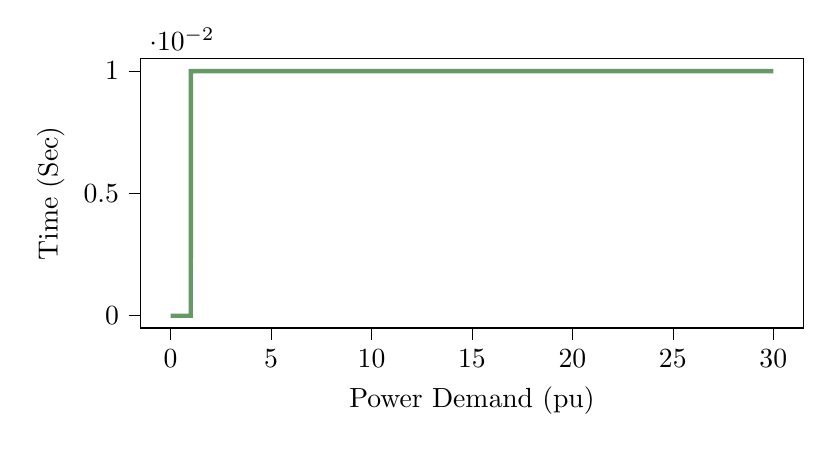
\begin{tikzpicture}

\definecolor{color0}{rgb}{0.12156862745098,0.466666666666667,0.705882352941177}

\begin{axis}[
compat=newest,
tick align=outside,
tick pos=left,
x grid style={white!69.0196078431373!black},
xmin=-1.50000000000009, xmax=31.500000000002,
xtick style={color=black},
y grid style={white!69.0196078431373!black},
ymin=-0.0005, ymax=0.0105,
ytick style={color=black},
scaled y ticks=true,
scaled y ticks=base 10:2,
width=10cm,
height=5cm,
xlabel=Power Demand (pu),
ylabel=Time (Sec)
]
\addplot [ultra thick, green!20!gray]
table {%
0 0
0.01 0
0.02 0
0.03 0
0.04 0
0.05 0
0.06 0
0.07 0
0.08 0
0.09 0
0.1 0
0.11 0
0.12 0
0.13 0
0.14 0
0.15 0
0.16 0
0.17 0
0.18 0
0.19 0
0.2 0
0.21 0
0.22 0
0.23 0
0.24 0
0.25 0
0.26 0
0.27 0
0.28 0
0.29 0
0.3 0
0.31 0
0.32 0
0.33 0
0.34 0
0.35 0
0.36 0
0.37 0
0.38 0
0.39 0
0.4 0
0.41 0
0.42 0
0.43 0
0.44 0
0.45 0
0.46 0
0.47 0
0.48 0
0.49 0
0.5 0
0.51 0
0.52 0
0.53 0
0.54 0
0.55 0
0.56 0
0.57 0
0.58 0
0.59 0
0.6 0
0.61 0
0.62 0
0.63 0
0.64 0
0.65 0
0.66 0
0.67 0
0.68 0
0.69 0
0.7 0
0.71 0
0.72 0
0.73 0
0.74 0
0.75 0
0.76 0
0.77 0
0.78 0
0.79 0
0.8 0
0.81 0
0.820000000000001 0
0.830000000000001 0
0.840000000000001 0
0.850000000000001 0
0.860000000000001 0
0.870000000000001 0
0.880000000000001 0
0.890000000000001 0
0.900000000000001 0
0.910000000000001 0
0.920000000000001 0
0.930000000000001 0
0.940000000000001 0
0.950000000000001 0
0.960000000000001 0
0.970000000000001 0
0.980000000000001 0
0.990000000000001 0
1 0
1.01 0.01
1.02 0.01
1.03 0.01
1.04 0.01
1.05 0.01
1.06 0.01
1.07 0.01
1.08 0.01
1.09 0.01
1.1 0.01
1.11 0.01
1.12 0.01
1.13 0.01
1.14 0.01
1.15 0.01
1.16 0.01
1.17 0.01
1.18 0.01
1.19 0.01
1.2 0.01
1.21 0.01
1.22 0.01
1.23 0.01
1.24 0.01
1.25 0.01
1.26 0.01
1.27 0.01
1.28 0.01
1.29 0.01
1.3 0.01
1.31 0.01
1.32 0.01
1.33 0.01
1.34 0.01
1.35 0.01
1.36 0.01
1.37 0.01
1.38 0.01
1.39 0.01
1.4 0.01
1.41 0.01
1.42 0.01
1.43 0.01
1.44 0.01
1.45 0.01
1.46 0.01
1.47 0.01
1.48 0.01
1.49 0.01
1.5 0.01
1.51 0.01
1.52 0.01
1.53 0.01
1.54 0.01
1.55 0.01
1.56 0.01
1.57 0.01
1.58 0.01
1.59 0.01
1.6 0.01
1.61 0.01
1.62 0.01
1.63 0.01
1.64 0.01
1.65 0.01
1.66 0.01
1.67 0.01
1.68 0.01
1.69 0.01
1.7 0.01
1.71 0.01
1.72 0.01
1.73 0.01
1.74 0.01
1.75 0.01
1.76 0.01
1.77 0.01
1.78 0.01
1.79 0.01
1.8 0.01
1.81 0.01
1.82 0.01
1.83 0.01
1.84 0.01
1.85 0.01
1.86 0.01
1.87 0.01
1.88 0.01
1.89 0.01
1.9 0.01
1.91 0.01
1.92 0.01
1.93 0.01
1.94 0.01
1.95 0.01
1.96 0.01
1.97 0.01
1.98 0.01
1.99 0.01
2 0.01
2.01 0.01
2.02 0.01
2.03 0.01
2.04 0.01
2.05 0.01
2.06 0.01
2.07 0.01
2.08 0.01
2.09 0.01
2.1 0.01
2.11 0.01
2.12 0.01
2.13 0.01
2.14 0.01
2.15 0.01
2.16 0.01
2.17 0.01
2.18 0.01
2.19 0.01
2.2 0.01
2.21 0.01
2.22 0.01
2.23 0.01
2.24 0.01
2.25 0.01
2.26 0.01
2.27 0.01
2.28 0.01
2.29 0.01
2.29999999999999 0.01
2.30999999999999 0.01
2.31999999999999 0.01
2.32999999999999 0.01
2.33999999999999 0.01
2.34999999999999 0.01
2.35999999999999 0.01
2.36999999999999 0.01
2.37999999999999 0.01
2.38999999999999 0.01
2.39999999999999 0.01
2.40999999999999 0.01
2.41999999999999 0.01
2.42999999999999 0.01
2.43999999999999 0.01
2.44999999999999 0.01
2.45999999999999 0.01
2.46999999999999 0.01
2.47999999999999 0.01
2.48999999999999 0.01
2.49999999999999 0.01
2.50999999999999 0.01
2.51999999999999 0.01
2.52999999999999 0.01
2.53999999999999 0.01
2.54999999999999 0.01
2.55999999999999 0.01
2.56999999999999 0.01
2.57999999999999 0.01
2.58999999999999 0.01
2.59999999999999 0.01
2.60999999999999 0.01
2.61999999999999 0.01
2.62999999999999 0.01
2.63999999999999 0.01
2.64999999999999 0.01
2.65999999999999 0.01
2.66999999999999 0.01
2.67999999999999 0.01
2.68999999999999 0.01
2.69999999999999 0.01
2.70999999999999 0.01
2.71999999999999 0.01
2.72999999999999 0.01
2.73999999999999 0.01
2.74999999999999 0.01
2.75999999999999 0.01
2.76999999999998 0.01
2.77999999999998 0.01
2.78999999999998 0.01
2.79999999999998 0.01
2.80999999999998 0.01
2.81999999999998 0.01
2.82999999999998 0.01
2.83999999999998 0.01
2.84999999999998 0.01
2.85999999999998 0.01
2.86999999999998 0.01
2.87999999999998 0.01
2.88999999999998 0.01
2.89999999999998 0.01
2.90999999999998 0.01
2.91999999999998 0.01
2.92999999999998 0.01
2.93999999999998 0.01
2.94999999999998 0.01
2.95999999999998 0.01
2.96999999999998 0.01
2.97999999999998 0.01
2.98999999999998 0.01
2.99999999999998 0.01
3.00999999999998 0.01
3.01999999999998 0.01
3.02999999999998 0.01
3.03999999999998 0.01
3.04999999999998 0.01
3.05999999999998 0.01
3.06999999999998 0.01
3.07999999999998 0.01
3.08999999999998 0.01
3.09999999999998 0.01
3.10999999999998 0.01
3.11999999999998 0.01
3.12999999999998 0.01
3.13999999999998 0.01
3.14999999999998 0.01
3.15999999999998 0.01
3.16999999999998 0.01
3.17999999999998 0.01
3.18999999999998 0.01
3.19999999999998 0.01
3.20999999999998 0.01
3.21999999999998 0.01
3.22999999999998 0.01
3.23999999999997 0.01
3.24999999999997 0.01
3.25999999999997 0.01
3.26999999999997 0.01
3.27999999999997 0.01
3.28999999999997 0.01
3.29999999999997 0.01
3.30999999999997 0.01
3.31999999999997 0.01
3.32999999999997 0.01
3.33999999999997 0.01
3.34999999999997 0.01
3.35999999999997 0.01
3.36999999999997 0.01
3.37999999999997 0.01
3.38999999999997 0.01
3.39999999999997 0.01
3.40999999999997 0.01
3.41999999999997 0.01
3.42999999999997 0.01
3.43999999999997 0.01
3.44999999999997 0.01
3.45999999999997 0.01
3.46999999999997 0.01
3.47999999999997 0.01
3.48999999999997 0.01
3.49999999999997 0.01
3.50999999999997 0.01
3.51999999999997 0.01
3.52999999999997 0.01
3.53999999999997 0.01
3.54999999999997 0.01
3.55999999999997 0.01
3.56999999999997 0.01
3.57999999999997 0.01
3.58999999999997 0.01
3.59999999999997 0.01
3.60999999999997 0.01
3.61999999999997 0.01
3.62999999999997 0.01
3.63999999999997 0.01
3.64999999999997 0.01
3.65999999999997 0.01
3.66999999999997 0.01
3.67999999999997 0.01
3.68999999999997 0.01
3.69999999999997 0.01
3.70999999999996 0.01
3.71999999999996 0.01
3.72999999999996 0.01
3.73999999999996 0.01
3.74999999999996 0.01
3.75999999999996 0.01
3.76999999999996 0.01
3.77999999999996 0.01
3.78999999999996 0.01
3.79999999999996 0.01
3.80999999999996 0.01
3.81999999999996 0.01
3.82999999999996 0.01
3.83999999999996 0.01
3.84999999999996 0.01
3.85999999999996 0.01
3.86999999999996 0.01
3.87999999999996 0.01
3.88999999999996 0.01
3.89999999999996 0.01
3.90999999999996 0.01
3.91999999999996 0.01
3.92999999999996 0.01
3.93999999999996 0.01
3.94999999999996 0.01
3.95999999999996 0.01
3.96999999999996 0.01
3.97999999999996 0.01
3.98999999999996 0.01
3.99999999999996 0.01
4.00999999999996 0.01
4.01999999999996 0.01
4.02999999999996 0.01
4.03999999999996 0.01
4.04999999999996 0.01
4.05999999999996 0.01
4.06999999999996 0.01
4.07999999999996 0.01
4.08999999999996 0.01
4.09999999999996 0.01
4.10999999999996 0.01
4.11999999999996 0.01
4.12999999999996 0.01
4.13999999999996 0.01
4.14999999999996 0.01
4.15999999999996 0.01
4.16999999999996 0.01
4.17999999999996 0.01
4.18999999999996 0.01
4.19999999999995 0.01
4.20999999999995 0.01
4.21999999999995 0.01
4.22999999999995 0.01
4.23999999999995 0.01
4.24999999999995 0.01
4.25999999999995 0.01
4.26999999999995 0.01
4.27999999999995 0.01
4.28999999999995 0.01
4.29999999999995 0.01
4.30999999999995 0.01
4.31999999999995 0.01
4.32999999999995 0.01
4.33999999999995 0.01
4.34999999999995 0.01
4.35999999999995 0.01
4.36999999999995 0.01
4.37999999999995 0.01
4.38999999999995 0.01
4.39999999999995 0.01
4.40999999999995 0.01
4.41999999999995 0.01
4.42999999999995 0.01
4.43999999999995 0.01
4.44999999999995 0.01
4.45999999999995 0.01
4.46999999999995 0.01
4.47999999999995 0.01
4.48999999999995 0.01
4.49999999999995 0.01
4.50999999999995 0.01
4.51999999999995 0.01
4.52999999999995 0.01
4.53999999999995 0.01
4.54999999999995 0.01
4.55999999999995 0.01
4.56999999999995 0.01
4.57999999999995 0.01
4.58999999999995 0.01
4.59999999999995 0.01
4.60999999999995 0.01
4.61999999999995 0.01
4.62999999999995 0.01
4.63999999999995 0.01
4.64999999999995 0.01
4.65999999999995 0.01
4.66999999999994 0.01
4.67999999999994 0.01
4.68999999999994 0.01
4.69999999999994 0.01
4.70999999999994 0.01
4.71999999999994 0.01
4.72999999999994 0.01
4.73999999999994 0.01
4.74999999999994 0.01
4.75999999999994 0.01
4.76999999999994 0.01
4.77999999999994 0.01
4.78999999999994 0.01
4.79999999999994 0.01
4.80999999999994 0.01
4.81999999999994 0.01
4.82999999999994 0.01
4.83999999999994 0.01
4.84999999999994 0.01
4.85999999999994 0.01
4.86999999999994 0.01
4.87999999999994 0.01
4.88999999999994 0.01
4.89999999999994 0.01
4.90999999999994 0.01
4.91999999999994 0.01
4.92999999999994 0.01
4.93999999999994 0.01
4.94999999999994 0.01
4.95999999999994 0.01
4.96999999999994 0.01
4.97999999999994 0.01
4.98999999999994 0.01
4.99999999999994 0.01
5.00999999999994 0.01
5.01999999999994 0.01
5.02999999999994 0.01
5.03999999999994 0.01
5.04999999999994 0.01
5.05999999999994 0.01
5.06999999999994 0.01
5.07999999999994 0.01
5.08999999999994 0.01
5.09999999999994 0.01
5.10999999999994 0.01
5.11999999999994 0.01
5.12999999999994 0.01
5.13999999999993 0.01
5.14999999999993 0.01
5.15999999999993 0.01
5.16999999999993 0.01
5.17999999999993 0.01
5.18999999999993 0.01
5.19999999999993 0.01
5.20999999999993 0.01
5.21999999999993 0.01
5.22999999999993 0.01
5.23999999999993 0.01
5.24999999999993 0.01
5.25999999999993 0.01
5.26999999999993 0.01
5.27999999999993 0.01
5.28999999999993 0.01
5.29999999999993 0.01
5.30999999999993 0.01
5.31999999999993 0.01
5.32999999999993 0.01
5.33999999999993 0.01
5.34999999999993 0.01
5.35999999999993 0.01
5.36999999999993 0.01
5.37999999999993 0.01
5.38999999999993 0.01
5.39999999999993 0.01
5.40999999999993 0.01
5.41999999999993 0.01
5.42999999999993 0.01
5.43999999999993 0.01
5.44999999999993 0.01
5.45999999999993 0.01
5.46999999999993 0.01
5.47999999999993 0.01
5.48999999999993 0.01
5.49999999999993 0.01
5.50999999999993 0.01
5.51999999999993 0.01
5.52999999999993 0.01
5.53999999999993 0.01
5.54999999999993 0.01
5.55999999999993 0.01
5.56999999999993 0.01
5.57999999999993 0.01
5.58999999999993 0.01
5.59999999999993 0.01
5.60999999999992 0.01
5.61999999999992 0.01
5.62999999999992 0.01
5.63999999999992 0.01
5.64999999999992 0.01
5.65999999999992 0.01
5.66999999999992 0.01
5.67999999999992 0.01
5.68999999999992 0.01
5.69999999999992 0.01
5.70999999999992 0.01
5.71999999999992 0.01
5.72999999999992 0.01
5.73999999999992 0.01
5.74999999999992 0.01
5.75999999999992 0.01
5.76999999999992 0.01
5.77999999999992 0.01
5.78999999999992 0.01
5.79999999999992 0.01
5.80999999999992 0.01
5.81999999999992 0.01
5.82999999999992 0.01
5.83999999999992 0.01
5.84999999999992 0.01
5.85999999999992 0.01
5.86999999999992 0.01
5.87999999999992 0.01
5.88999999999992 0.01
5.89999999999992 0.01
5.90999999999992 0.01
5.91999999999992 0.01
5.92999999999992 0.01
5.93999999999992 0.01
5.94999999999992 0.01
5.95999999999992 0.01
5.96999999999992 0.01
5.97999999999992 0.01
5.98999999999992 0.01
5.99999999999992 0.01
6.00999999999992 0.01
6.01999999999992 0.01
6.02999999999992 0.01
6.03999999999992 0.01
6.04999999999992 0.01
6.05999999999992 0.01
6.06999999999992 0.01
6.07999999999991 0.01
6.08999999999991 0.01
6.09999999999991 0.01
6.10999999999991 0.01
6.11999999999991 0.01
6.12999999999991 0.01
6.13999999999991 0.01
6.14999999999991 0.01
6.15999999999991 0.01
6.16999999999991 0.01
6.17999999999991 0.01
6.18999999999991 0.01
6.19999999999991 0.01
6.20999999999991 0.01
6.21999999999991 0.01
6.22999999999991 0.01
6.23999999999991 0.01
6.24999999999991 0.01
6.25999999999991 0.01
6.26999999999991 0.01
6.27999999999991 0.01
6.28999999999991 0.01
6.29999999999991 0.01
6.30999999999991 0.01
6.31999999999991 0.01
6.32999999999991 0.01
6.33999999999991 0.01
6.34999999999991 0.01
6.35999999999991 0.01
6.36999999999991 0.01
6.37999999999991 0.01
6.38999999999991 0.01
6.39999999999991 0.01
6.40999999999991 0.01
6.41999999999991 0.01
6.42999999999991 0.01
6.43999999999991 0.01
6.44999999999991 0.01
6.45999999999991 0.01
6.46999999999991 0.01
6.47999999999991 0.01
6.48999999999991 0.01
6.49999999999991 0.01
6.50999999999991 0.01
6.51999999999991 0.01
6.52999999999991 0.01
6.53999999999991 0.01
6.5499999999999 0.01
6.5599999999999 0.01
6.5699999999999 0.01
6.5799999999999 0.01
6.5899999999999 0.01
6.5999999999999 0.01
6.6099999999999 0.01
6.6199999999999 0.01
6.6299999999999 0.01
6.6399999999999 0.01
6.6499999999999 0.01
6.6599999999999 0.01
6.6699999999999 0.01
6.6799999999999 0.01
6.6899999999999 0.01
6.6999999999999 0.01
6.7099999999999 0.01
6.7199999999999 0.01
6.7299999999999 0.01
6.7399999999999 0.01
6.7499999999999 0.01
6.7599999999999 0.01
6.7699999999999 0.01
6.7799999999999 0.01
6.7899999999999 0.01
6.7999999999999 0.01
6.8099999999999 0.01
6.8199999999999 0.01
6.8299999999999 0.01
6.8399999999999 0.01
6.8499999999999 0.01
6.8599999999999 0.01
6.8699999999999 0.01
6.8799999999999 0.01
6.8899999999999 0.01
6.8999999999999 0.01
6.9099999999999 0.01
6.9199999999999 0.01
6.9299999999999 0.01
6.9399999999999 0.01
6.9499999999999 0.01
6.9599999999999 0.01
6.9699999999999 0.01
6.9799999999999 0.01
6.9899999999999 0.01
6.9999999999999 0.01
7.00999999999989 0.01
7.01999999999989 0.01
7.02999999999989 0.01
7.03999999999989 0.01
7.04999999999989 0.01
7.05999999999989 0.01
7.06999999999989 0.01
7.07999999999989 0.01
7.08999999999989 0.01
7.09999999999989 0.01
7.10999999999989 0.01
7.11999999999989 0.01
7.12999999999989 0.01
7.13999999999989 0.01
7.14999999999989 0.01
7.15999999999989 0.01
7.16999999999989 0.01
7.17999999999989 0.01
7.18999999999989 0.01
7.19999999999989 0.01
7.20999999999989 0.01
7.21999999999989 0.01
7.22999999999989 0.01
7.23999999999989 0.01
7.24999999999989 0.01
7.25999999999989 0.01
7.26999999999989 0.01
7.27999999999989 0.01
7.28999999999989 0.01
7.29999999999989 0.01
7.30999999999989 0.01
7.31999999999989 0.01
7.32999999999989 0.01
7.33999999999989 0.01
7.34999999999989 0.01
7.35999999999989 0.01
7.36999999999989 0.01
7.37999999999989 0.01
7.38999999999989 0.01
7.39999999999989 0.01
7.40999999999989 0.01
7.41999999999989 0.01
7.42999999999989 0.01
7.43999999999989 0.01
7.44999999999989 0.01
7.45999999999989 0.01
7.46999999999989 0.01
7.47999999999988 0.01
7.48999999999988 0.01
7.49999999999988 0.01
7.50999999999988 0.01
7.51999999999988 0.01
7.52999999999988 0.01
7.53999999999988 0.01
7.54999999999988 0.01
7.55999999999988 0.01
7.56999999999988 0.01
7.57999999999988 0.01
7.58999999999988 0.01
7.59999999999988 0.01
7.60999999999988 0.01
7.61999999999988 0.01
7.62999999999988 0.01
7.63999999999988 0.01
7.64999999999988 0.01
7.65999999999988 0.01
7.66999999999988 0.01
7.67999999999988 0.01
7.68999999999988 0.01
7.69999999999988 0.01
7.70999999999988 0.01
7.71999999999988 0.01
7.72999999999988 0.01
7.73999999999988 0.01
7.74999999999988 0.01
7.75999999999988 0.01
7.76999999999988 0.01
7.77999999999988 0.01
7.78999999999988 0.01
7.79999999999988 0.01
7.80999999999988 0.01
7.81999999999988 0.01
7.82999999999988 0.01
7.83999999999988 0.01
7.84999999999988 0.01
7.85999999999988 0.01
7.86999999999988 0.01
7.87999999999988 0.01
7.88999999999988 0.01
7.89999999999988 0.01
7.90999999999988 0.01
7.91999999999988 0.01
7.92999999999988 0.01
7.93999999999988 0.01
7.94999999999987 0.01
7.95999999999987 0.01
7.96999999999987 0.01
7.97999999999987 0.01
7.98999999999987 0.01
7.99999999999987 0.01
8.00999999999987 0.01
8.01999999999987 0.01
8.02999999999987 0.01
8.03999999999987 0.01
8.04999999999987 0.01
8.05999999999987 0.01
8.06999999999987 0.01
8.07999999999987 0.01
8.08999999999987 0.01
8.09999999999987 0.01
8.10999999999987 0.01
8.11999999999987 0.01
8.12999999999987 0.01
8.13999999999987 0.01
8.14999999999987 0.01
8.15999999999987 0.01
8.16999999999987 0.01
8.17999999999987 0.01
8.18999999999987 0.01
8.19999999999987 0.01
8.20999999999987 0.01
8.21999999999987 0.01
8.22999999999987 0.01
8.23999999999987 0.01
8.24999999999987 0.01
8.25999999999987 0.01
8.26999999999987 0.01
8.27999999999987 0.01
8.28999999999987 0.01
8.29999999999987 0.01
8.30999999999987 0.01
8.31999999999987 0.01
8.32999999999987 0.01
8.33999999999987 0.01
8.34999999999987 0.01
8.35999999999987 0.01
8.36999999999987 0.01
8.37999999999987 0.01
8.38999999999987 0.01
8.39999999999987 0.01
8.40999999999987 0.01
8.41999999999986 0.01
8.42999999999986 0.01
8.43999999999986 0.01
8.44999999999986 0.01
8.45999999999986 0.01
8.46999999999986 0.01
8.47999999999986 0.01
8.48999999999986 0.01
8.49999999999986 0.01
8.50999999999986 0.01
8.51999999999986 0.01
8.52999999999986 0.01
8.53999999999986 0.01
8.54999999999986 0.01
8.55999999999986 0.01
8.56999999999986 0.01
8.57999999999986 0.01
8.58999999999986 0.01
8.59999999999986 0.01
8.60999999999986 0.01
8.61999999999986 0.01
8.62999999999986 0.01
8.63999999999986 0.01
8.64999999999986 0.01
8.65999999999986 0.01
8.66999999999986 0.01
8.67999999999986 0.01
8.68999999999986 0.01
8.69999999999986 0.01
8.70999999999986 0.01
8.71999999999986 0.01
8.72999999999986 0.01
8.73999999999986 0.01
8.74999999999986 0.01
8.75999999999986 0.01
8.76999999999986 0.01
8.77999999999986 0.01
8.78999999999986 0.01
8.79999999999986 0.01
8.80999999999986 0.01
8.81999999999986 0.01
8.82999999999986 0.01
8.83999999999986 0.01
8.84999999999986 0.01
8.85999999999986 0.01
8.86999999999986 0.01
8.87999999999986 0.01
8.88999999999985 0.01
8.89999999999985 0.01
8.90999999999985 0.01
8.91999999999985 0.01
8.92999999999985 0.01
8.93999999999985 0.01
8.94999999999985 0.01
8.95999999999985 0.01
8.96999999999985 0.01
8.97999999999985 0.01
8.98999999999985 0.01
8.99999999999985 0.01
9.00999999999985 0.01
9.01999999999985 0.01
9.02999999999985 0.01
9.03999999999985 0.01
9.04999999999985 0.01
9.05999999999985 0.01
9.06999999999985 0.01
9.07999999999985 0.01
9.08999999999985 0.01
9.09999999999985 0.01
9.10999999999985 0.01
9.11999999999985 0.01
9.12999999999985 0.01
9.13999999999985 0.01
9.14999999999985 0.01
9.15999999999985 0.01
9.16999999999985 0.01
9.17999999999985 0.01
9.18999999999985 0.01
9.19999999999985 0.01
9.20999999999985 0.01
9.21999999999985 0.01
9.22999999999985 0.01
9.23999999999985 0.01
9.24999999999985 0.01
9.25999999999985 0.01
9.26999999999985 0.01
9.27999999999985 0.01
9.28999999999985 0.01
9.29999999999985 0.01
9.30999999999985 0.01
9.31999999999985 0.01
9.32999999999985 0.01
9.33999999999985 0.01
9.34999999999985 0.01
9.35999999999984 0.01
9.36999999999984 0.01
9.37999999999984 0.01
9.38999999999984 0.01
9.39999999999984 0.01
9.40999999999984 0.01
9.41999999999984 0.01
9.42999999999984 0.01
9.43999999999984 0.01
9.44999999999984 0.01
9.45999999999984 0.01
9.46999999999984 0.01
9.47999999999984 0.01
9.48999999999984 0.01
9.49999999999984 0.01
9.50999999999984 0.01
9.51999999999984 0.01
9.52999999999984 0.01
9.53999999999984 0.01
9.54999999999984 0.01
9.55999999999984 0.01
9.56999999999984 0.01
9.57999999999984 0.01
9.58999999999984 0.01
9.59999999999984 0.01
9.60999999999984 0.01
9.61999999999984 0.01
9.62999999999984 0.01
9.63999999999984 0.01
9.64999999999984 0.01
9.65999999999984 0.01
9.66999999999984 0.01
9.67999999999984 0.01
9.68999999999984 0.01
9.69999999999984 0.01
9.70999999999984 0.01
9.71999999999984 0.01
9.72999999999984 0.01
9.73999999999984 0.01
9.74999999999984 0.01
9.75999999999984 0.01
9.76999999999984 0.01
9.77999999999984 0.01
9.78999999999984 0.01
9.79999999999984 0.01
9.80999999999984 0.01
9.81999999999984 0.01
9.82999999999983 0.01
9.83999999999983 0.01
9.84999999999983 0.01
9.85999999999983 0.01
9.86999999999983 0.01
9.87999999999983 0.01
9.88999999999983 0.01
9.89999999999983 0.01
9.90999999999983 0.01
9.91999999999983 0.01
9.92999999999983 0.01
9.93999999999983 0.01
9.94999999999983 0.01
9.95999999999983 0.01
9.96999999999983 0.01
9.97999999999983 0.01
9.98999999999983 0.01
9.99999999999983 0.01
10.0099999999998 0.01
10.0199999999998 0.01
10.0299999999998 0.01
10.0399999999998 0.01
10.0499999999998 0.01
10.0599999999998 0.01
10.0699999999998 0.01
10.0799999999998 0.01
10.0899999999998 0.01
10.0999999999998 0.01
10.1099999999998 0.01
10.1199999999998 0.01
10.1299999999998 0.01
10.1399999999998 0.01
10.1499999999998 0.01
10.1599999999998 0.01
10.1699999999998 0.01
10.1799999999998 0.01
10.1899999999998 0.01
10.1999999999998 0.01
10.2099999999998 0.01
10.2199999999998 0.01
10.2299999999998 0.01
10.2399999999998 0.01
10.2499999999998 0.01
10.2599999999998 0.01
10.2699999999998 0.01
10.2799999999998 0.01
10.2899999999998 0.01
10.2999999999998 0.01
10.3099999999998 0.01
10.3199999999998 0.01
10.3299999999998 0.01
10.3399999999998 0.01
10.3499999999998 0.01
10.3599999999998 0.01
10.3699999999998 0.01
10.3799999999998 0.01
10.3899999999998 0.01
10.3999999999998 0.01
10.4099999999998 0.01
10.4199999999998 0.01
10.4299999999998 0.01
10.4399999999998 0.01
10.4499999999998 0.01
10.4599999999998 0.01
10.4699999999998 0.01
10.4799999999998 0.01
10.4899999999998 0.01
10.4999999999998 0.01
10.5099999999998 0.01
10.5199999999998 0.01
10.5299999999998 0.01
10.5399999999998 0.01
10.5499999999998 0.01
10.5599999999998 0.01
10.5699999999998 0.01
10.5799999999998 0.01
10.5899999999998 0.01
10.5999999999998 0.01
10.6099999999998 0.01
10.6199999999998 0.01
10.6299999999998 0.01
10.6399999999998 0.01
10.6499999999998 0.01
10.6599999999998 0.01
10.6699999999998 0.01
10.6799999999998 0.01
10.6899999999998 0.01
10.6999999999998 0.01
10.7099999999998 0.01
10.7199999999998 0.01
10.7299999999998 0.01
10.7399999999998 0.01
10.7499999999998 0.01
10.7599999999998 0.01
10.7699999999998 0.01
10.7799999999998 0.01
10.7899999999998 0.01
10.7999999999998 0.01
10.8099999999998 0.01
10.8199999999998 0.01
10.8299999999998 0.01
10.8399999999998 0.01
10.8499999999998 0.01
10.8599999999998 0.01
10.8699999999998 0.01
10.8799999999998 0.01
10.8899999999998 0.01
10.8999999999998 0.01
10.9099999999998 0.01
10.9199999999998 0.01
10.9299999999998 0.01
10.9399999999998 0.01
10.9499999999998 0.01
10.9599999999998 0.01
10.9699999999998 0.01
10.9799999999998 0.01
10.9899999999998 0.01
10.9999999999998 0.01
11.0099999999998 0.01
11.0199999999998 0.01
11.0299999999998 0.01
11.0399999999998 0.01
11.0499999999998 0.01
11.0599999999998 0.01
11.0699999999998 0.01
11.0799999999998 0.01
11.0899999999998 0.01
11.0999999999998 0.01
11.1099999999998 0.01
11.1199999999998 0.01
11.1299999999998 0.01
11.1399999999998 0.01
11.1499999999998 0.01
11.1599999999998 0.01
11.1699999999998 0.01
11.1799999999998 0.01
11.1899999999998 0.01
11.1999999999998 0.01
11.2099999999998 0.01
11.2199999999998 0.01
11.2299999999998 0.01
11.2399999999998 0.01
11.2499999999998 0.01
11.2599999999998 0.01
11.2699999999998 0.01
11.2799999999998 0.01
11.2899999999998 0.01
11.2999999999998 0.01
11.3099999999998 0.01
11.3199999999998 0.01
11.3299999999998 0.01
11.3399999999998 0.01
11.3499999999998 0.01
11.3599999999998 0.01
11.3699999999998 0.01
11.3799999999998 0.01
11.3899999999998 0.01
11.3999999999998 0.01
11.4099999999998 0.01
11.4199999999998 0.01
11.4299999999998 0.01
11.4399999999998 0.01
11.4499999999998 0.01
11.4599999999998 0.01
11.4699999999998 0.01
11.4799999999998 0.01
11.4899999999998 0.01
11.4999999999998 0.01
11.5099999999998 0.01
11.5199999999998 0.01
11.5299999999998 0.01
11.5399999999998 0.01
11.5499999999998 0.01
11.5599999999998 0.01
11.5699999999998 0.01
11.5799999999998 0.01
11.5899999999998 0.01
11.5999999999998 0.01
11.6099999999998 0.01
11.6199999999998 0.01
11.6299999999998 0.01
11.6399999999998 0.01
11.6499999999998 0.01
11.6599999999998 0.01
11.6699999999998 0.01
11.6799999999998 0.01
11.6899999999998 0.01
11.6999999999998 0.01
11.7099999999998 0.01
11.7199999999998 0.01
11.7299999999998 0.01
11.7399999999998 0.01
11.7499999999998 0.01
11.7599999999998 0.01
11.7699999999998 0.01
11.7799999999998 0.01
11.7899999999998 0.01
11.7999999999998 0.01
11.8099999999998 0.01
11.8199999999998 0.01
11.8299999999998 0.01
11.8399999999998 0.01
11.8499999999998 0.01
11.8599999999998 0.01
11.8699999999998 0.01
11.8799999999998 0.01
11.8899999999998 0.01
11.8999999999998 0.01
11.9099999999998 0.01
11.9199999999998 0.01
11.9299999999998 0.01
11.9399999999998 0.01
11.9499999999998 0.01
11.9599999999998 0.01
11.9699999999998 0.01
11.9799999999998 0.01
11.9899999999998 0.01
11.9999999999998 0.01
12.0099999999998 0.01
12.0199999999998 0.01
12.0299999999998 0.01
12.0399999999998 0.01
12.0499999999998 0.01
12.0599999999998 0.01
12.0699999999998 0.01
12.0799999999998 0.01
12.0899999999998 0.01
12.0999999999998 0.01
12.1099999999998 0.01
12.1199999999998 0.01
12.1299999999998 0.01
12.1399999999998 0.01
12.1499999999998 0.01
12.1599999999998 0.01
12.1699999999998 0.01
12.1799999999998 0.01
12.1899999999998 0.01
12.1999999999998 0.01
12.2099999999998 0.01
12.2199999999998 0.01
12.2299999999998 0.01
12.2399999999998 0.01
12.2499999999998 0.01
12.2599999999998 0.01
12.2699999999998 0.01
12.2799999999998 0.01
12.2899999999998 0.01
12.2999999999998 0.01
12.3099999999998 0.01
12.3199999999998 0.01
12.3299999999998 0.01
12.3399999999998 0.01
12.3499999999998 0.01
12.3599999999998 0.01
12.3699999999998 0.01
12.3799999999998 0.01
12.3899999999998 0.01
12.3999999999998 0.01
12.4099999999998 0.01
12.4199999999998 0.01
12.4299999999998 0.01
12.4399999999998 0.01
12.4499999999998 0.01
12.4599999999998 0.01
12.4699999999998 0.01
12.4799999999998 0.01
12.4899999999998 0.01
12.4999999999998 0.01
12.5099999999998 0.01
12.5199999999998 0.01
12.5299999999998 0.01
12.5399999999998 0.01
12.5499999999998 0.01
12.5599999999998 0.01
12.5699999999998 0.01
12.5799999999998 0.01
12.5899999999998 0.01
12.5999999999998 0.01
12.6099999999998 0.01
12.6199999999998 0.01
12.6299999999998 0.01
12.6399999999998 0.01
12.6499999999998 0.01
12.6599999999998 0.01
12.6699999999998 0.01
12.6799999999998 0.01
12.6899999999998 0.01
12.6999999999998 0.01
12.7099999999998 0.01
12.7199999999998 0.01
12.7299999999998 0.01
12.7399999999998 0.01
12.7499999999998 0.01
12.7599999999998 0.01
12.7699999999998 0.01
12.7799999999998 0.01
12.7899999999998 0.01
12.7999999999998 0.01
12.8099999999998 0.01
12.8199999999998 0.01
12.8299999999998 0.01
12.8399999999998 0.01
12.8499999999998 0.01
12.8599999999998 0.01
12.8699999999998 0.01
12.8799999999998 0.01
12.8899999999998 0.01
12.8999999999998 0.01
12.9099999999998 0.01
12.9199999999998 0.01
12.9299999999998 0.01
12.9399999999998 0.01
12.9499999999998 0.01
12.9599999999998 0.01
12.9699999999998 0.01
12.9799999999998 0.01
12.9899999999998 0.01
12.9999999999998 0.01
13.0099999999998 0.01
13.0199999999998 0.01
13.0299999999998 0.01
13.0399999999998 0.01
13.0499999999998 0.01
13.0599999999998 0.01
13.0699999999998 0.01
13.0799999999998 0.01
13.0899999999998 0.01
13.0999999999998 0.01
13.1099999999998 0.01
13.1199999999998 0.01
13.1299999999998 0.01
13.1399999999998 0.01
13.1499999999998 0.01
13.1599999999998 0.01
13.1699999999998 0.01
13.1799999999998 0.01
13.1899999999998 0.01
13.1999999999998 0.01
13.2099999999998 0.01
13.2199999999998 0.01
13.2299999999998 0.01
13.2399999999998 0.01
13.2499999999998 0.01
13.2599999999998 0.01
13.2699999999998 0.01
13.2799999999998 0.01
13.2899999999998 0.01
13.2999999999998 0.01
13.3099999999998 0.01
13.3199999999998 0.01
13.3299999999998 0.01
13.3399999999998 0.01
13.3499999999998 0.01
13.3599999999998 0.01
13.3699999999998 0.01
13.3799999999998 0.01
13.3899999999998 0.01
13.3999999999998 0.01
13.4099999999998 0.01
13.4199999999998 0.01
13.4299999999998 0.01
13.4399999999998 0.01
13.4499999999998 0.01
13.4599999999998 0.01
13.4699999999998 0.01
13.4799999999998 0.01
13.4899999999998 0.01
13.4999999999998 0.01
13.5099999999998 0.01
13.5199999999998 0.01
13.5299999999998 0.01
13.5399999999998 0.01
13.5499999999998 0.01
13.5599999999998 0.01
13.5699999999998 0.01
13.5799999999998 0.01
13.5899999999998 0.01
13.5999999999998 0.01
13.6099999999998 0.01
13.6199999999998 0.01
13.6299999999998 0.01
13.6399999999998 0.01
13.6499999999998 0.01
13.6599999999998 0.01
13.6699999999998 0.01
13.6799999999998 0.01
13.6899999999998 0.01
13.6999999999998 0.01
13.7099999999998 0.01
13.7199999999998 0.01
13.7299999999998 0.01
13.7399999999998 0.01
13.7499999999998 0.01
13.7599999999998 0.01
13.7699999999998 0.01
13.7799999999998 0.01
13.7899999999998 0.01
13.7999999999998 0.01
13.8099999999998 0.01
13.8199999999997 0.01
13.8299999999997 0.01
13.8399999999997 0.01
13.8499999999997 0.01
13.8599999999997 0.01
13.8699999999997 0.01
13.8799999999997 0.01
13.8899999999997 0.01
13.8999999999997 0.01
13.9099999999997 0.01
13.9199999999997 0.01
13.9299999999997 0.01
13.9399999999997 0.01
13.9499999999997 0.01
13.9599999999997 0.01
13.9699999999997 0.01
13.9799999999997 0.01
13.9899999999997 0.01
13.9999999999997 0.01
14.0099999999997 0.01
14.0199999999997 0.01
14.0299999999997 0.01
14.0399999999997 0.01
14.0499999999997 0.01
14.0599999999997 0.01
14.0699999999997 0.01
14.0799999999997 0.01
14.0899999999997 0.01
14.0999999999997 0.01
14.1099999999997 0.01
14.1199999999997 0.01
14.1299999999997 0.01
14.1399999999997 0.01
14.1499999999997 0.01
14.1599999999997 0.01
14.1699999999997 0.01
14.1799999999997 0.01
14.1899999999997 0.01
14.1999999999997 0.01
14.2099999999997 0.01
14.2199999999997 0.01
14.2299999999997 0.01
14.2399999999997 0.01
14.2499999999997 0.01
14.2599999999997 0.01
14.2699999999997 0.01
14.2799999999997 0.01
14.2899999999997 0.01
14.2999999999997 0.01
14.3099999999997 0.01
14.3199999999997 0.01
14.3299999999997 0.01
14.3399999999997 0.01
14.3499999999997 0.01
14.3599999999997 0.01
14.3699999999997 0.01
14.3799999999997 0.01
14.3899999999997 0.01
14.3999999999997 0.01
14.4099999999997 0.01
14.4199999999997 0.01
14.4299999999997 0.01
14.4399999999997 0.01
14.4499999999997 0.01
14.4599999999997 0.01
14.4699999999997 0.01
14.4799999999997 0.01
14.4899999999997 0.01
14.4999999999997 0.01
14.5099999999997 0.01
14.5199999999997 0.01
14.5299999999997 0.01
14.5399999999997 0.01
14.5499999999997 0.01
14.5599999999997 0.01
14.5699999999997 0.01
14.5799999999997 0.01
14.5899999999997 0.01
14.5999999999997 0.01
14.6099999999997 0.01
14.6199999999997 0.01
14.6299999999997 0.01
14.6399999999997 0.01
14.6499999999997 0.01
14.6599999999997 0.01
14.6699999999997 0.01
14.6799999999997 0.01
14.6899999999997 0.01
14.6999999999997 0.01
14.7099999999997 0.01
14.7199999999997 0.01
14.7299999999997 0.01
14.7399999999997 0.01
14.7499999999997 0.01
14.7599999999997 0.01
14.7699999999997 0.01
14.7799999999997 0.01
14.7899999999997 0.01
14.7999999999997 0.01
14.8099999999997 0.01
14.8199999999997 0.01
14.8299999999997 0.01
14.8399999999997 0.01
14.8499999999997 0.01
14.8599999999997 0.01
14.8699999999997 0.01
14.8799999999997 0.01
14.8899999999997 0.01
14.8999999999997 0.01
14.9099999999997 0.01
14.9199999999997 0.01
14.9299999999997 0.01
14.9399999999997 0.01
14.9499999999997 0.01
14.9599999999997 0.01
14.9699999999997 0.01
14.9799999999997 0.01
14.9899999999997 0.01
14.9999999999997 0.01
15.0099999999997 0.01
15.0199999999997 0.01
15.0299999999997 0.01
15.0399999999997 0.01
15.0499999999997 0.01
15.0599999999997 0.01
15.0699999999997 0.01
15.0799999999997 0.01
15.0899999999997 0.01
15.0999999999997 0.01
15.1099999999997 0.01
15.1199999999997 0.01
15.1299999999997 0.01
15.1399999999997 0.01
15.1499999999997 0.01
15.1599999999997 0.01
15.1699999999997 0.01
15.1799999999997 0.01
15.1899999999997 0.01
15.1999999999997 0.01
15.2099999999997 0.01
15.2199999999997 0.01
15.2299999999997 0.01
15.2399999999997 0.01
15.2499999999997 0.01
15.2599999999997 0.01
15.2699999999997 0.01
15.2799999999997 0.01
15.2899999999997 0.01
15.2999999999997 0.01
15.3099999999997 0.01
15.3199999999997 0.01
15.3299999999997 0.01
15.3399999999997 0.01
15.3499999999997 0.01
15.3599999999997 0.01
15.3699999999997 0.01
15.3799999999997 0.01
15.3899999999997 0.01
15.3999999999997 0.01
15.4099999999997 0.01
15.4199999999997 0.01
15.4299999999997 0.01
15.4399999999997 0.01
15.4499999999997 0.01
15.4599999999997 0.01
15.4699999999997 0.01
15.4799999999997 0.01
15.4899999999997 0.01
15.4999999999997 0.01
15.5099999999997 0.01
15.5199999999997 0.01
15.5299999999997 0.01
15.5399999999997 0.01
15.5499999999997 0.01
15.5599999999997 0.01
15.5699999999997 0.01
15.5799999999997 0.01
15.5899999999997 0.01
15.5999999999997 0.01
15.6099999999997 0.01
15.6199999999997 0.01
15.6299999999997 0.01
15.6399999999997 0.01
15.6499999999997 0.01
15.6599999999997 0.01
15.6699999999997 0.01
15.6799999999997 0.01
15.6899999999997 0.01
15.6999999999997 0.01
15.7099999999997 0.01
15.7199999999997 0.01
15.7299999999997 0.01
15.7399999999997 0.01
15.7499999999997 0.01
15.7599999999997 0.01
15.7699999999997 0.01
15.7799999999997 0.01
15.7899999999997 0.01
15.7999999999997 0.01
15.8099999999997 0.01
15.8199999999997 0.01
15.8299999999997 0.01
15.8399999999997 0.01
15.8499999999997 0.01
15.8599999999997 0.01
15.8699999999997 0.01
15.8799999999997 0.01
15.8899999999997 0.01
15.8999999999997 0.01
15.9099999999997 0.01
15.9199999999997 0.01
15.9299999999997 0.01
15.9399999999997 0.01
15.9499999999997 0.01
15.9599999999997 0.01
15.9699999999997 0.01
15.9799999999997 0.01
15.9899999999997 0.01
15.9999999999997 0.01
16.0099999999997 0.01
16.0199999999997 0.01
16.0299999999997 0.01
16.0399999999997 0.01
16.0499999999997 0.01
16.0599999999997 0.01
16.0699999999997 0.01
16.0799999999997 0.01
16.0899999999997 0.01
16.0999999999997 0.01
16.1099999999997 0.01
16.1199999999997 0.01
16.1299999999997 0.01
16.1399999999997 0.01
16.1499999999997 0.01
16.1599999999997 0.01
16.1699999999997 0.01
16.1799999999997 0.01
16.1899999999997 0.01
16.1999999999997 0.01
16.2099999999997 0.01
16.2199999999997 0.01
16.2299999999997 0.01
16.2399999999997 0.01
16.2499999999997 0.01
16.2599999999997 0.01
16.2699999999997 0.01
16.2799999999997 0.01
16.2899999999997 0.01
16.2999999999997 0.01
16.3099999999998 0.01
16.3199999999998 0.01
16.3299999999998 0.01
16.3399999999998 0.01
16.3499999999998 0.01
16.3599999999998 0.01
16.3699999999998 0.01
16.3799999999998 0.01
16.3899999999998 0.01
16.3999999999998 0.01
16.4099999999998 0.01
16.4199999999998 0.01
16.4299999999998 0.01
16.4399999999998 0.01
16.4499999999998 0.01
16.4599999999998 0.01
16.4699999999998 0.01
16.4799999999998 0.01
16.4899999999998 0.01
16.4999999999998 0.01
16.5099999999998 0.01
16.5199999999998 0.01
16.5299999999998 0.01
16.5399999999998 0.01
16.5499999999998 0.01
16.5599999999998 0.01
16.5699999999998 0.01
16.5799999999998 0.01
16.5899999999998 0.01
16.5999999999998 0.01
16.6099999999998 0.01
16.6199999999998 0.01
16.6299999999998 0.01
16.6399999999998 0.01
16.6499999999998 0.01
16.6599999999998 0.01
16.6699999999998 0.01
16.6799999999998 0.01
16.6899999999998 0.01
16.6999999999998 0.01
16.7099999999998 0.01
16.7199999999998 0.01
16.7299999999998 0.01
16.7399999999998 0.01
16.7499999999998 0.01
16.7599999999998 0.01
16.7699999999998 0.01
16.7799999999998 0.01
16.7899999999998 0.01
16.7999999999998 0.01
16.8099999999998 0.01
16.8199999999998 0.01
16.8299999999998 0.01
16.8399999999998 0.01
16.8499999999998 0.01
16.8599999999998 0.01
16.8699999999998 0.01
16.8799999999998 0.01
16.8899999999998 0.01
16.8999999999998 0.01
16.9099999999998 0.01
16.9199999999998 0.01
16.9299999999998 0.01
16.9399999999998 0.01
16.9499999999999 0.01
16.9599999999999 0.01
16.9699999999999 0.01
16.9799999999999 0.01
16.9899999999999 0.01
16.9999999999999 0.01
17.0099999999999 0.01
17.0199999999999 0.01
17.0299999999999 0.01
17.0399999999999 0.01
17.0499999999999 0.01
17.0599999999999 0.01
17.0699999999999 0.01
17.0799999999999 0.01
17.0899999999999 0.01
17.0999999999999 0.01
17.1099999999999 0.01
17.1199999999999 0.01
17.1299999999999 0.01
17.1399999999999 0.01
17.1499999999999 0.01
17.1599999999999 0.01
17.1699999999999 0.01
17.1799999999999 0.01
17.1899999999999 0.01
17.1999999999999 0.01
17.2099999999999 0.01
17.2199999999999 0.01
17.2299999999999 0.01
17.2399999999999 0.01
17.2499999999999 0.01
17.2599999999999 0.01
17.2699999999999 0.01
17.2799999999999 0.01
17.2899999999999 0.01
17.2999999999999 0.01
17.3099999999999 0.01
17.3199999999999 0.01
17.3299999999999 0.01
17.3399999999999 0.01
17.3499999999999 0.01
17.3599999999999 0.01
17.3699999999999 0.01
17.3799999999999 0.01
17.3899999999999 0.01
17.3999999999999 0.01
17.4099999999999 0.01
17.4199999999999 0.01
17.4299999999999 0.01
17.4399999999999 0.01
17.4499999999999 0.01
17.4599999999999 0.01
17.4699999999999 0.01
17.4799999999999 0.01
17.4899999999999 0.01
17.4999999999999 0.01
17.5099999999999 0.01
17.5199999999999 0.01
17.5299999999999 0.01
17.5399999999999 0.01
17.5499999999999 0.01
17.5599999999999 0.01
17.5699999999999 0.01
17.5799999999999 0.01
17.59 0.01
17.6 0.01
17.61 0.01
17.62 0.01
17.63 0.01
17.64 0.01
17.65 0.01
17.66 0.01
17.67 0.01
17.68 0.01
17.69 0.01
17.7 0.01
17.71 0.01
17.72 0.01
17.73 0.01
17.74 0.01
17.75 0.01
17.76 0.01
17.77 0.01
17.78 0.01
17.79 0.01
17.8 0.01
17.81 0.01
17.82 0.01
17.83 0.01
17.84 0.01
17.85 0.01
17.86 0.01
17.87 0.01
17.88 0.01
17.89 0.01
17.9 0.01
17.91 0.01
17.92 0.01
17.93 0.01
17.94 0.01
17.95 0.01
17.96 0.01
17.97 0.01
17.98 0.01
17.99 0.01
18 0.01
18.01 0.01
18.02 0.01
18.03 0.01
18.04 0.01
18.05 0.01
18.06 0.01
18.07 0.01
18.08 0.01
18.09 0.01
18.1 0.01
18.11 0.01
18.12 0.01
18.13 0.01
18.14 0.01
18.15 0.01
18.16 0.01
18.17 0.01
18.18 0.01
18.19 0.01
18.2 0.01
18.21 0.01
18.22 0.01
18.2300000000001 0.01
18.2400000000001 0.01
18.2500000000001 0.01
18.2600000000001 0.01
18.2700000000001 0.01
18.2800000000001 0.01
18.2900000000001 0.01
18.3000000000001 0.01
18.3100000000001 0.01
18.3200000000001 0.01
18.3300000000001 0.01
18.3400000000001 0.01
18.3500000000001 0.01
18.3600000000001 0.01
18.3700000000001 0.01
18.3800000000001 0.01
18.3900000000001 0.01
18.4000000000001 0.01
18.4100000000001 0.01
18.4200000000001 0.01
18.4300000000001 0.01
18.4400000000001 0.01
18.4500000000001 0.01
18.4600000000001 0.01
18.4700000000001 0.01
18.4800000000001 0.01
18.4900000000001 0.01
18.5000000000001 0.01
18.5100000000001 0.01
18.5200000000001 0.01
18.5300000000001 0.01
18.5400000000001 0.01
18.5500000000001 0.01
18.5600000000001 0.01
18.5700000000001 0.01
18.5800000000001 0.01
18.5900000000001 0.01
18.6000000000001 0.01
18.6100000000001 0.01
18.6200000000001 0.01
18.6300000000001 0.01
18.6400000000001 0.01
18.6500000000001 0.01
18.6600000000001 0.01
18.6700000000001 0.01
18.6800000000001 0.01
18.6900000000001 0.01
18.7000000000001 0.01
18.7100000000001 0.01
18.7200000000001 0.01
18.7300000000001 0.01
18.7400000000001 0.01
18.7500000000001 0.01
18.7600000000001 0.01
18.7700000000001 0.01
18.7800000000001 0.01
18.7900000000001 0.01
18.8000000000001 0.01
18.8100000000001 0.01
18.8200000000001 0.01
18.8300000000001 0.01
18.8400000000001 0.01
18.8500000000001 0.01
18.8600000000001 0.01
18.8700000000002 0.01
18.8800000000002 0.01
18.8900000000002 0.01
18.9000000000002 0.01
18.9100000000002 0.01
18.9200000000002 0.01
18.9300000000002 0.01
18.9400000000002 0.01
18.9500000000002 0.01
18.9600000000002 0.01
18.9700000000002 0.01
18.9800000000002 0.01
18.9900000000002 0.01
19.0000000000002 0.01
19.0100000000002 0.01
19.0200000000002 0.01
19.0300000000002 0.01
19.0400000000002 0.01
19.0500000000002 0.01
19.0600000000002 0.01
19.0700000000002 0.01
19.0800000000002 0.01
19.0900000000002 0.01
19.1000000000002 0.01
19.1100000000002 0.01
19.1200000000002 0.01
19.1300000000002 0.01
19.1400000000002 0.01
19.1500000000002 0.01
19.1600000000002 0.01
19.1700000000002 0.01
19.1800000000002 0.01
19.1900000000002 0.01
19.2000000000002 0.01
19.2100000000002 0.01
19.2200000000002 0.01
19.2300000000002 0.01
19.2400000000002 0.01
19.2500000000002 0.01
19.2600000000002 0.01
19.2700000000002 0.01
19.2800000000002 0.01
19.2900000000002 0.01
19.3000000000002 0.01
19.3100000000002 0.01
19.3200000000002 0.01
19.3300000000002 0.01
19.3400000000002 0.01
19.3500000000002 0.01
19.3600000000002 0.01
19.3700000000002 0.01
19.3800000000002 0.01
19.3900000000002 0.01
19.4000000000002 0.01
19.4100000000002 0.01
19.4200000000002 0.01
19.4300000000002 0.01
19.4400000000002 0.01
19.4500000000002 0.01
19.4600000000002 0.01
19.4700000000002 0.01
19.4800000000002 0.01
19.4900000000002 0.01
19.5000000000002 0.01
19.5100000000003 0.01
19.5200000000003 0.01
19.5300000000003 0.01
19.5400000000003 0.01
19.5500000000003 0.01
19.5600000000003 0.01
19.5700000000003 0.01
19.5800000000003 0.01
19.5900000000003 0.01
19.6000000000003 0.01
19.6100000000003 0.01
19.6200000000003 0.01
19.6300000000003 0.01
19.6400000000003 0.01
19.6500000000003 0.01
19.6600000000003 0.01
19.6700000000003 0.01
19.6800000000003 0.01
19.6900000000003 0.01
19.7000000000003 0.01
19.7100000000003 0.01
19.7200000000003 0.01
19.7300000000003 0.01
19.7400000000003 0.01
19.7500000000003 0.01
19.7600000000003 0.01
19.7700000000003 0.01
19.7800000000003 0.01
19.7900000000003 0.01
19.8000000000003 0.01
19.8100000000003 0.01
19.8200000000003 0.01
19.8300000000003 0.01
19.8400000000003 0.01
19.8500000000003 0.01
19.8600000000003 0.01
19.8700000000003 0.01
19.8800000000003 0.01
19.8900000000003 0.01
19.9000000000003 0.01
19.9100000000003 0.01
19.9200000000003 0.01
19.9300000000003 0.01
19.9400000000003 0.01
19.9500000000003 0.01
19.9600000000003 0.01
19.9700000000003 0.01
19.9800000000003 0.01
19.9900000000003 0.01
20.0000000000003 0.01
20.0100000000003 0.01
20.0200000000003 0.01
20.0300000000003 0.01
20.0400000000003 0.01
20.0500000000003 0.01
20.0600000000003 0.01
20.0700000000003 0.01
20.0800000000003 0.01
20.0900000000003 0.01
20.1000000000003 0.01
20.1100000000003 0.01
20.1200000000003 0.01
20.1300000000003 0.01
20.1400000000003 0.01
20.1500000000004 0.01
20.1600000000004 0.01
20.1700000000004 0.01
20.1800000000004 0.01
20.1900000000004 0.01
20.2000000000004 0.01
20.2100000000004 0.01
20.2200000000004 0.01
20.2300000000004 0.01
20.2400000000004 0.01
20.2500000000004 0.01
20.2600000000004 0.01
20.2700000000004 0.01
20.2800000000004 0.01
20.2900000000004 0.01
20.3000000000004 0.01
20.3100000000004 0.01
20.3200000000004 0.01
20.3300000000004 0.01
20.3400000000004 0.01
20.3500000000004 0.01
20.3600000000004 0.01
20.3700000000004 0.01
20.3800000000004 0.01
20.3900000000004 0.01
20.4000000000004 0.01
20.4100000000004 0.01
20.4200000000004 0.01
20.4300000000004 0.01
20.4400000000004 0.01
20.4500000000004 0.01
20.4600000000004 0.01
20.4700000000004 0.01
20.4800000000004 0.01
20.4900000000004 0.01
20.5000000000004 0.01
20.5100000000004 0.01
20.5200000000004 0.01
20.5300000000004 0.01
20.5400000000004 0.01
20.5500000000004 0.01
20.5600000000004 0.01
20.5700000000004 0.01
20.5800000000004 0.01
20.5900000000004 0.01
20.6000000000004 0.01
20.6100000000004 0.01
20.6200000000004 0.01
20.6300000000004 0.01
20.6400000000004 0.01
20.6500000000004 0.01
20.6600000000004 0.01
20.6700000000004 0.01
20.6800000000004 0.01
20.6900000000004 0.01
20.7000000000004 0.01
20.7100000000004 0.01
20.7200000000004 0.01
20.7300000000004 0.01
20.7400000000004 0.01
20.7500000000004 0.01
20.7600000000004 0.01
20.7700000000004 0.01
20.7800000000004 0.01
20.7900000000005 0.01
20.8000000000005 0.01
20.8100000000005 0.01
20.8200000000005 0.01
20.8300000000005 0.01
20.8400000000005 0.01
20.8500000000005 0.01
20.8600000000005 0.01
20.8700000000005 0.01
20.8800000000005 0.01
20.8900000000005 0.01
20.9000000000005 0.01
20.9100000000005 0.01
20.9200000000005 0.01
20.9300000000005 0.01
20.9400000000005 0.01
20.9500000000005 0.01
20.9600000000005 0.01
20.9700000000005 0.01
20.9800000000005 0.01
20.9900000000005 0.01
21.0000000000005 0.01
21.0100000000005 0.01
21.0200000000005 0.01
21.0300000000005 0.01
21.0400000000005 0.01
21.0500000000005 0.01
21.0600000000005 0.01
21.0700000000005 0.01
21.0800000000005 0.01
21.0900000000005 0.01
21.1000000000005 0.01
21.1100000000005 0.01
21.1200000000005 0.01
21.1300000000005 0.01
21.1400000000005 0.01
21.1500000000005 0.01
21.1600000000005 0.01
21.1700000000005 0.01
21.1800000000005 0.01
21.1900000000005 0.01
21.2000000000005 0.01
21.2100000000005 0.01
21.2200000000005 0.01
21.2300000000005 0.01
21.2400000000005 0.01
21.2500000000005 0.01
21.2600000000005 0.01
21.2700000000005 0.01
21.2800000000005 0.01
21.2900000000005 0.01
21.3000000000005 0.01
21.3100000000005 0.01
21.3200000000005 0.01
21.3300000000005 0.01
21.3400000000005 0.01
21.3500000000005 0.01
21.3600000000005 0.01
21.3700000000005 0.01
21.3800000000005 0.01
21.3900000000005 0.01
21.4000000000005 0.01
21.4100000000005 0.01
21.4200000000005 0.01
21.4300000000006 0.01
21.4400000000006 0.01
21.4500000000006 0.01
21.4600000000006 0.01
21.4700000000006 0.01
21.4800000000006 0.01
21.4900000000006 0.01
21.5000000000006 0.01
21.5100000000006 0.01
21.5200000000006 0.01
21.5300000000006 0.01
21.5400000000006 0.01
21.5500000000006 0.01
21.5600000000006 0.01
21.5700000000006 0.01
21.5800000000006 0.01
21.5900000000006 0.01
21.6000000000006 0.01
21.6100000000006 0.01
21.6200000000006 0.01
21.6300000000006 0.01
21.6400000000006 0.01
21.6500000000006 0.01
21.6600000000006 0.01
21.6700000000006 0.01
21.6800000000006 0.01
21.6900000000006 0.01
21.7000000000006 0.01
21.7100000000006 0.01
21.7200000000006 0.01
21.7300000000006 0.01
21.7400000000006 0.01
21.7500000000006 0.01
21.7600000000006 0.01
21.7700000000006 0.01
21.7800000000006 0.01
21.7900000000006 0.01
21.8000000000006 0.01
21.8100000000006 0.01
21.8200000000006 0.01
21.8300000000006 0.01
21.8400000000006 0.01
21.8500000000006 0.01
21.8600000000006 0.01
21.8700000000006 0.01
21.8800000000006 0.01
21.8900000000006 0.01
21.9000000000006 0.01
21.9100000000006 0.01
21.9200000000006 0.01
21.9300000000006 0.01
21.9400000000006 0.01
21.9500000000006 0.01
21.9600000000006 0.01
21.9700000000006 0.01
21.9800000000006 0.01
21.9900000000006 0.01
22.0000000000006 0.01
22.0100000000006 0.01
22.0200000000006 0.01
22.0300000000006 0.01
22.0400000000006 0.01
22.0500000000006 0.01
22.0600000000006 0.01
22.0700000000007 0.01
22.0800000000007 0.01
22.0900000000007 0.01
22.1000000000007 0.01
22.1100000000007 0.01
22.1200000000007 0.01
22.1300000000007 0.01
22.1400000000007 0.01
22.1500000000007 0.01
22.1600000000007 0.01
22.1700000000007 0.01
22.1800000000007 0.01
22.1900000000007 0.01
22.2000000000007 0.01
22.2100000000007 0.01
22.2200000000007 0.01
22.2300000000007 0.01
22.2400000000007 0.01
22.2500000000007 0.01
22.2600000000007 0.01
22.2700000000007 0.01
22.2800000000007 0.01
22.2900000000007 0.01
22.3000000000007 0.01
22.3100000000007 0.01
22.3200000000007 0.01
22.3300000000007 0.01
22.3400000000007 0.01
22.3500000000007 0.01
22.3600000000007 0.01
22.3700000000007 0.01
22.3800000000007 0.01
22.3900000000007 0.01
22.4000000000007 0.01
22.4100000000007 0.01
22.4200000000007 0.01
22.4300000000007 0.01
22.4400000000007 0.01
22.4500000000007 0.01
22.4600000000007 0.01
22.4700000000007 0.01
22.4800000000007 0.01
22.4900000000007 0.01
22.5000000000007 0.01
22.5100000000007 0.01
22.5200000000007 0.01
22.5300000000007 0.01
22.5400000000007 0.01
22.5500000000007 0.01
22.5600000000007 0.01
22.5700000000007 0.01
22.5800000000007 0.01
22.5900000000007 0.01
22.6000000000007 0.01
22.6100000000007 0.01
22.6200000000007 0.01
22.6300000000007 0.01
22.6400000000007 0.01
22.6500000000007 0.01
22.6600000000007 0.01
22.6700000000007 0.01
22.6800000000007 0.01
22.6900000000007 0.01
22.7000000000007 0.01
22.7100000000008 0.01
22.7200000000008 0.01
22.7300000000008 0.01
22.7400000000008 0.01
22.7500000000008 0.01
22.7600000000008 0.01
22.7700000000008 0.01
22.7800000000008 0.01
22.7900000000008 0.01
22.8000000000008 0.01
22.8100000000008 0.01
22.8200000000008 0.01
22.8300000000008 0.01
22.8400000000008 0.01
22.8500000000008 0.01
22.8600000000008 0.01
22.8700000000008 0.01
22.8800000000008 0.01
22.8900000000008 0.01
22.9000000000008 0.01
22.9100000000008 0.01
22.9200000000008 0.01
22.9300000000008 0.01
22.9400000000008 0.01
22.9500000000008 0.01
22.9600000000008 0.01
22.9700000000008 0.01
22.9800000000008 0.01
22.9900000000008 0.01
23.0000000000008 0.01
23.0100000000008 0.01
23.0200000000008 0.01
23.0300000000008 0.01
23.0400000000008 0.01
23.0500000000008 0.01
23.0600000000008 0.01
23.0700000000008 0.01
23.0800000000008 0.01
23.0900000000008 0.01
23.1000000000008 0.01
23.1100000000008 0.01
23.1200000000008 0.01
23.1300000000008 0.01
23.1400000000008 0.01
23.1500000000008 0.01
23.1600000000008 0.01
23.1700000000008 0.01
23.1800000000008 0.01
23.1900000000008 0.01
23.2000000000008 0.01
23.2100000000008 0.01
23.2200000000008 0.01
23.2300000000008 0.01
23.2400000000008 0.01
23.2500000000008 0.01
23.2600000000008 0.01
23.2700000000008 0.01
23.2800000000008 0.01
23.2900000000008 0.01
23.3000000000008 0.01
23.3100000000008 0.01
23.3200000000008 0.01
23.3300000000008 0.01
23.3400000000008 0.01
23.3500000000009 0.01
23.3600000000009 0.01
23.3700000000009 0.01
23.3800000000009 0.01
23.3900000000009 0.01
23.4000000000009 0.01
23.4100000000009 0.01
23.4200000000009 0.01
23.4300000000009 0.01
23.4400000000009 0.01
23.4500000000009 0.01
23.4600000000009 0.01
23.4700000000009 0.01
23.4800000000009 0.01
23.4900000000009 0.01
23.5000000000009 0.01
23.5100000000009 0.01
23.5200000000009 0.01
23.5300000000009 0.01
23.5400000000009 0.01
23.5500000000009 0.01
23.5600000000009 0.01
23.5700000000009 0.01
23.5800000000009 0.01
23.5900000000009 0.01
23.6000000000009 0.01
23.6100000000009 0.01
23.6200000000009 0.01
23.6300000000009 0.01
23.6400000000009 0.01
23.6500000000009 0.01
23.6600000000009 0.01
23.6700000000009 0.01
23.6800000000009 0.01
23.6900000000009 0.01
23.7000000000009 0.01
23.7100000000009 0.01
23.7200000000009 0.01
23.7300000000009 0.01
23.7400000000009 0.01
23.7500000000009 0.01
23.7600000000009 0.01
23.7700000000009 0.01
23.7800000000009 0.01
23.7900000000009 0.01
23.8000000000009 0.01
23.8100000000009 0.01
23.8200000000009 0.01
23.8300000000009 0.01
23.8400000000009 0.01
23.8500000000009 0.01
23.8600000000009 0.01
23.8700000000009 0.01
23.8800000000009 0.01
23.8900000000009 0.01
23.9000000000009 0.01
23.9100000000009 0.01
23.9200000000009 0.01
23.9300000000009 0.01
23.9400000000009 0.01
23.9500000000009 0.01
23.9600000000009 0.01
23.9700000000009 0.01
23.9800000000009 0.01
23.990000000001 0.01
24.000000000001 0.01
24.010000000001 0.01
24.020000000001 0.01
24.030000000001 0.01
24.040000000001 0.01
24.050000000001 0.01
24.060000000001 0.01
24.070000000001 0.01
24.080000000001 0.01
24.090000000001 0.01
24.100000000001 0.01
24.110000000001 0.01
24.120000000001 0.01
24.130000000001 0.01
24.140000000001 0.01
24.150000000001 0.01
24.160000000001 0.01
24.170000000001 0.01
24.180000000001 0.01
24.190000000001 0.01
24.200000000001 0.01
24.210000000001 0.01
24.220000000001 0.01
24.230000000001 0.01
24.240000000001 0.01
24.250000000001 0.01
24.260000000001 0.01
24.270000000001 0.01
24.280000000001 0.01
24.290000000001 0.01
24.300000000001 0.01
24.310000000001 0.01
24.320000000001 0.01
24.330000000001 0.01
24.340000000001 0.01
24.350000000001 0.01
24.360000000001 0.01
24.370000000001 0.01
24.380000000001 0.01
24.390000000001 0.01
24.400000000001 0.01
24.410000000001 0.01
24.420000000001 0.01
24.430000000001 0.01
24.440000000001 0.01
24.450000000001 0.01
24.460000000001 0.01
24.470000000001 0.01
24.480000000001 0.01
24.490000000001 0.01
24.500000000001 0.01
24.510000000001 0.01
24.520000000001 0.01
24.530000000001 0.01
24.540000000001 0.01
24.550000000001 0.01
24.560000000001 0.01
24.570000000001 0.01
24.580000000001 0.01
24.590000000001 0.01
24.600000000001 0.01
24.610000000001 0.01
24.620000000001 0.01
24.6300000000011 0.01
24.6400000000011 0.01
24.6500000000011 0.01
24.6600000000011 0.01
24.6700000000011 0.01
24.6800000000011 0.01
24.6900000000011 0.01
24.7000000000011 0.01
24.7100000000011 0.01
24.7200000000011 0.01
24.7300000000011 0.01
24.7400000000011 0.01
24.7500000000011 0.01
24.7600000000011 0.01
24.7700000000011 0.01
24.7800000000011 0.01
24.7900000000011 0.01
24.8000000000011 0.01
24.8100000000011 0.01
24.8200000000011 0.01
24.8300000000011 0.01
24.8400000000011 0.01
24.8500000000011 0.01
24.8600000000011 0.01
24.8700000000011 0.01
24.8800000000011 0.01
24.8900000000011 0.01
24.9000000000011 0.01
24.9100000000011 0.01
24.9200000000011 0.01
24.9300000000011 0.01
24.9400000000011 0.01
24.9500000000011 0.01
24.9600000000011 0.01
24.9700000000011 0.01
24.9800000000011 0.01
24.9900000000011 0.01
25.0000000000011 0.01
25.0100000000011 0.01
25.0200000000011 0.01
25.0300000000011 0.01
25.0400000000011 0.01
25.0500000000011 0.01
25.0600000000011 0.01
25.0700000000011 0.01
25.0800000000011 0.01
25.0900000000011 0.01
25.1000000000011 0.01
25.1100000000011 0.01
25.1200000000011 0.01
25.1300000000011 0.01
25.1400000000011 0.01
25.1500000000011 0.01
25.1600000000011 0.01
25.1700000000011 0.01
25.1800000000011 0.01
25.1900000000011 0.01
25.2000000000011 0.01
25.2100000000011 0.01
25.2200000000011 0.01
25.2300000000011 0.01
25.2400000000011 0.01
25.2500000000011 0.01
25.2600000000011 0.01
25.2700000000012 0.01
25.2800000000012 0.01
25.2900000000012 0.01
25.3000000000012 0.01
25.3100000000012 0.01
25.3200000000012 0.01
25.3300000000012 0.01
25.3400000000012 0.01
25.3500000000012 0.01
25.3600000000012 0.01
25.3700000000012 0.01
25.3800000000012 0.01
25.3900000000012 0.01
25.4000000000012 0.01
25.4100000000012 0.01
25.4200000000012 0.01
25.4300000000012 0.01
25.4400000000012 0.01
25.4500000000012 0.01
25.4600000000012 0.01
25.4700000000012 0.01
25.4800000000012 0.01
25.4900000000012 0.01
25.5000000000012 0.01
25.5100000000012 0.01
25.5200000000012 0.01
25.5300000000012 0.01
25.5400000000012 0.01
25.5500000000012 0.01
25.5600000000012 0.01
25.5700000000012 0.01
25.5800000000012 0.01
25.5900000000012 0.01
25.6000000000012 0.01
25.6100000000012 0.01
25.6200000000012 0.01
25.6300000000012 0.01
25.6400000000012 0.01
25.6500000000012 0.01
25.6600000000012 0.01
25.6700000000012 0.01
25.6800000000012 0.01
25.6900000000012 0.01
25.7000000000012 0.01
25.7100000000012 0.01
25.7200000000012 0.01
25.7300000000012 0.01
25.7400000000012 0.01
25.7500000000012 0.01
25.7600000000012 0.01
25.7700000000012 0.01
25.7800000000012 0.01
25.7900000000012 0.01
25.8000000000012 0.01
25.8100000000012 0.01
25.8200000000012 0.01
25.8300000000012 0.01
25.8400000000012 0.01
25.8500000000012 0.01
25.8600000000012 0.01
25.8700000000012 0.01
25.8800000000012 0.01
25.8900000000012 0.01
25.9000000000012 0.01
25.9100000000013 0.01
25.9200000000013 0.01
25.9300000000013 0.01
25.9400000000013 0.01
25.9500000000013 0.01
25.9600000000013 0.01
25.9700000000013 0.01
25.9800000000013 0.01
25.9900000000013 0.01
26.0000000000013 0.01
26.0100000000013 0.01
26.0200000000013 0.01
26.0300000000013 0.01
26.0400000000013 0.01
26.0500000000013 0.01
26.0600000000013 0.01
26.0700000000013 0.01
26.0800000000013 0.01
26.0900000000013 0.01
26.1000000000013 0.01
26.1100000000013 0.01
26.1200000000013 0.01
26.1300000000013 0.01
26.1400000000013 0.01
26.1500000000013 0.01
26.1600000000013 0.01
26.1700000000013 0.01
26.1800000000013 0.01
26.1900000000013 0.01
26.2000000000013 0.01
26.2100000000013 0.01
26.2200000000013 0.01
26.2300000000013 0.01
26.2400000000013 0.01
26.2500000000013 0.01
26.2600000000013 0.01
26.2700000000013 0.01
26.2800000000013 0.01
26.2900000000013 0.01
26.3000000000013 0.01
26.3100000000013 0.01
26.3200000000013 0.01
26.3300000000013 0.01
26.3400000000013 0.01
26.3500000000013 0.01
26.3600000000013 0.01
26.3700000000013 0.01
26.3800000000013 0.01
26.3900000000013 0.01
26.4000000000013 0.01
26.4100000000013 0.01
26.4200000000013 0.01
26.4300000000013 0.01
26.4400000000013 0.01
26.4500000000013 0.01
26.4600000000013 0.01
26.4700000000013 0.01
26.4800000000013 0.01
26.4900000000013 0.01
26.5000000000013 0.01
26.5100000000013 0.01
26.5200000000013 0.01
26.5300000000013 0.01
26.5400000000013 0.01
26.5500000000014 0.01
26.5600000000014 0.01
26.5700000000014 0.01
26.5800000000014 0.01
26.5900000000014 0.01
26.6000000000014 0.01
26.6100000000014 0.01
26.6200000000014 0.01
26.6300000000014 0.01
26.6400000000014 0.01
26.6500000000014 0.01
26.6600000000014 0.01
26.6700000000014 0.01
26.6800000000014 0.01
26.6900000000014 0.01
26.7000000000014 0.01
26.7100000000014 0.01
26.7200000000014 0.01
26.7300000000014 0.01
26.7400000000014 0.01
26.7500000000014 0.01
26.7600000000014 0.01
26.7700000000014 0.01
26.7800000000014 0.01
26.7900000000014 0.01
26.8000000000014 0.01
26.8100000000014 0.01
26.8200000000014 0.01
26.8300000000014 0.01
26.8400000000014 0.01
26.8500000000014 0.01
26.8600000000014 0.01
26.8700000000014 0.01
26.8800000000014 0.01
26.8900000000014 0.01
26.9000000000014 0.01
26.9100000000014 0.01
26.9200000000014 0.01
26.9300000000014 0.01
26.9400000000014 0.01
26.9500000000014 0.01
26.9600000000014 0.01
26.9700000000014 0.01
26.9800000000014 0.01
26.9900000000014 0.01
27.0000000000014 0.01
27.0100000000014 0.01
27.0200000000014 0.01
27.0300000000014 0.01
27.0400000000014 0.01
27.0500000000014 0.01
27.0600000000014 0.01
27.0700000000014 0.01
27.0800000000014 0.01
27.0900000000014 0.01
27.1000000000014 0.01
27.1100000000014 0.01
27.1200000000014 0.01
27.1300000000014 0.01
27.1400000000014 0.01
27.1500000000014 0.01
27.1600000000014 0.01
27.1700000000014 0.01
27.1800000000014 0.01
27.1900000000015 0.01
27.2000000000015 0.01
27.2100000000015 0.01
27.2200000000015 0.01
27.2300000000015 0.01
27.2400000000015 0.01
27.2500000000015 0.01
27.2600000000015 0.01
27.2700000000015 0.01
27.2800000000015 0.01
27.2900000000015 0.01
27.3000000000015 0.01
27.3100000000015 0.01
27.3200000000015 0.01
27.3300000000015 0.01
27.3400000000015 0.01
27.3500000000015 0.01
27.3600000000015 0.01
27.3700000000015 0.01
27.3800000000015 0.01
27.3900000000015 0.01
27.4000000000015 0.01
27.4100000000015 0.01
27.4200000000015 0.01
27.4300000000015 0.01
27.4400000000015 0.01
27.4500000000015 0.01
27.4600000000015 0.01
27.4700000000015 0.01
27.4800000000015 0.01
27.4900000000015 0.01
27.5000000000015 0.01
27.5100000000015 0.01
27.5200000000015 0.01
27.5300000000015 0.01
27.5400000000015 0.01
27.5500000000015 0.01
27.5600000000015 0.01
27.5700000000015 0.01
27.5800000000015 0.01
27.5900000000015 0.01
27.6000000000015 0.01
27.6100000000015 0.01
27.6200000000015 0.01
27.6300000000015 0.01
27.6400000000015 0.01
27.6500000000015 0.01
27.6600000000015 0.01
27.6700000000015 0.01
27.6800000000015 0.01
27.6900000000015 0.01
27.7000000000015 0.01
27.7100000000015 0.01
27.7200000000015 0.01
27.7300000000015 0.01
27.7400000000015 0.01
27.7500000000015 0.01
27.7600000000015 0.01
27.7700000000015 0.01
27.7800000000015 0.01
27.7900000000015 0.01
27.8000000000015 0.01
27.8100000000015 0.01
27.8200000000015 0.01
27.8300000000016 0.01
27.8400000000016 0.01
27.8500000000016 0.01
27.8600000000016 0.01
27.8700000000016 0.01
27.8800000000016 0.01
27.8900000000016 0.01
27.9000000000016 0.01
27.9100000000016 0.01
27.9200000000016 0.01
27.9300000000016 0.01
27.9400000000016 0.01
27.9500000000016 0.01
27.9600000000016 0.01
27.9700000000016 0.01
27.9800000000016 0.01
27.9900000000016 0.01
28.0000000000016 0.01
28.0100000000016 0.01
28.0200000000016 0.01
28.0300000000016 0.01
28.0400000000016 0.01
28.0500000000016 0.01
28.0600000000016 0.01
28.0700000000016 0.01
28.0800000000016 0.01
28.0900000000016 0.01
28.1000000000016 0.01
28.1100000000016 0.01
28.1200000000016 0.01
28.1300000000016 0.01
28.1400000000016 0.01
28.1500000000016 0.01
28.1600000000016 0.01
28.1700000000016 0.01
28.1800000000016 0.01
28.1900000000016 0.01
28.2000000000016 0.01
28.2100000000016 0.01
28.2200000000016 0.01
28.2300000000016 0.01
28.2400000000016 0.01
28.2500000000016 0.01
28.2600000000016 0.01
28.2700000000016 0.01
28.2800000000016 0.01
28.2900000000016 0.01
28.3000000000016 0.01
28.3100000000016 0.01
28.3200000000016 0.01
28.3300000000016 0.01
28.3400000000016 0.01
28.3500000000016 0.01
28.3600000000016 0.01
28.3700000000016 0.01
28.3800000000016 0.01
28.3900000000016 0.01
28.4000000000016 0.01
28.4100000000016 0.01
28.4200000000016 0.01
28.4300000000016 0.01
28.4400000000016 0.01
28.4500000000016 0.01
28.4600000000016 0.01
28.4700000000017 0.01
28.4800000000017 0.01
28.4900000000017 0.01
28.5000000000017 0.01
28.5100000000017 0.01
28.5200000000017 0.01
28.5300000000017 0.01
28.5400000000017 0.01
28.5500000000017 0.01
28.5600000000017 0.01
28.5700000000017 0.01
28.5800000000017 0.01
28.5900000000017 0.01
28.6000000000017 0.01
28.6100000000017 0.01
28.6200000000017 0.01
28.6300000000017 0.01
28.6400000000017 0.01
28.6500000000017 0.01
28.6600000000017 0.01
28.6700000000017 0.01
28.6800000000017 0.01
28.6900000000017 0.01
28.7000000000017 0.01
28.7100000000017 0.01
28.7200000000017 0.01
28.7300000000017 0.01
28.7400000000017 0.01
28.7500000000017 0.01
28.7600000000017 0.01
28.7700000000017 0.01
28.7800000000017 0.01
28.7900000000017 0.01
28.8000000000017 0.01
28.8100000000017 0.01
28.8200000000017 0.01
28.8300000000017 0.01
28.8400000000017 0.01
28.8500000000017 0.01
28.8600000000017 0.01
28.8700000000017 0.01
28.8800000000017 0.01
28.8900000000017 0.01
28.9000000000017 0.01
28.9100000000017 0.01
28.9200000000017 0.01
28.9300000000017 0.01
28.9400000000017 0.01
28.9500000000017 0.01
28.9600000000017 0.01
28.9700000000017 0.01
28.9800000000017 0.01
28.9900000000017 0.01
29.0000000000017 0.01
29.0100000000017 0.01
29.0200000000017 0.01
29.0300000000017 0.01
29.0400000000017 0.01
29.0500000000017 0.01
29.0600000000017 0.01
29.0700000000017 0.01
29.0800000000017 0.01
29.0900000000017 0.01
29.1000000000017 0.01
29.1100000000018 0.01
29.1200000000018 0.01
29.1300000000018 0.01
29.1400000000018 0.01
29.1500000000018 0.01
29.1600000000018 0.01
29.1700000000018 0.01
29.1800000000018 0.01
29.1900000000018 0.01
29.2000000000018 0.01
29.2100000000018 0.01
29.2200000000018 0.01
29.2300000000018 0.01
29.2400000000018 0.01
29.2500000000018 0.01
29.2600000000018 0.01
29.2700000000018 0.01
29.2800000000018 0.01
29.2900000000018 0.01
29.3000000000018 0.01
29.3100000000018 0.01
29.3200000000018 0.01
29.3300000000018 0.01
29.3400000000018 0.01
29.3500000000018 0.01
29.3600000000018 0.01
29.3700000000018 0.01
29.3800000000018 0.01
29.3900000000018 0.01
29.4000000000018 0.01
29.4100000000018 0.01
29.4200000000018 0.01
29.4300000000018 0.01
29.4400000000018 0.01
29.4500000000018 0.01
29.4600000000018 0.01
29.4700000000018 0.01
29.4800000000018 0.01
29.4900000000018 0.01
29.5000000000018 0.01
29.5100000000018 0.01
29.5200000000018 0.01
29.5300000000018 0.01
29.5400000000018 0.01
29.5500000000018 0.01
29.5600000000018 0.01
29.5700000000018 0.01
29.5800000000018 0.01
29.5900000000018 0.01
29.6000000000018 0.01
29.6100000000018 0.01
29.6200000000018 0.01
29.6300000000018 0.01
29.6400000000018 0.01
29.6500000000018 0.01
29.6600000000018 0.01
29.6700000000018 0.01
29.6800000000018 0.01
29.6900000000018 0.01
29.7000000000018 0.01
29.7100000000018 0.01
29.7200000000018 0.01
29.7300000000018 0.01
29.7400000000018 0.01
29.7500000000019 0.01
29.7600000000019 0.01
29.7700000000019 0.01
29.7800000000019 0.01
29.7900000000019 0.01
29.8000000000019 0.01
29.8100000000019 0.01
29.8200000000019 0.01
29.8300000000019 0.01
29.8400000000019 0.01
29.8500000000019 0.01
29.8600000000019 0.01
29.8700000000019 0.01
29.8800000000019 0.01
29.8900000000019 0.01
29.9000000000019 0.01
29.9100000000019 0.01
29.9200000000019 0.01
29.9300000000019 0.01
29.9400000000019 0.01
29.9500000000019 0.01
29.9600000000019 0.01
29.9700000000019 0.01
29.9800000000019 0.01
29.9900000000019 0.01
30.0000000000019 0.01
};
\end{axis}

\end{tikzpicture}

	\caption[Preliminary investigation load demand step change]{At the 1 sec mark the system experiences a step load change in the power demand in Area 1, and the simulation continues for 30 sec thereafter.}
	\label{fig:5001_demand_profile}
\end{figure}

From initialisation, the simulation was incrementally stepped forward by 0.01 sec for a total of 3000 steps. At each time step the DDPG agent was trained using experience stored in the replay buffer from current and previous system interactions, for a given experiment. Experiments were allowed to run for a total of 10000 episodes.

DDPG training algorithm hyperparameters were held constant for each experiment, as per the values used originally by Lillicrap \textit{et alias} \cite{Lillicrap2015}. Hyperparameter values used for the experiments described in this chapter are documented in Table \ref{tab:5000_hyperparameters}.

\begin{table}[h]
	\centering
	\caption{DDPG hyperparameters used for preliminary investigation experiments.}
	\begin{tabular}{lrlr}
	\toprule
	\textbf{Hyperparameter} & \textbf{Value} & \textbf{Hyperparameter} & \textbf{Value} \\
	\midrule
	Buffer Size 	 & $1 \times 10^6$  & Batch Size 	& 256 \\
	Gamma ($\gamma$) & 0.99 	& Tau ($\tau$) 	& $1 \times 10^{-3}$ \\
	Actor Learning Rate ($\alpha_{\texttt{actor}}$) & $1 \times 10^{-4}$ & Critic Learning Rate ($\alpha_{\texttt{critic}}$) & $3 \times 10^{-4} $ \\
	Weight Decay & 0.00 & & \\
	\bottomrule
	\end{tabular}\label{tab:5000_hyperparameters}
\end{table}

Each experiment, detailed in the remaining sections of this chapter, modified a single variable of the agent construction, holding other variables constant. and cumulative reward for each episode. for each power system area were captured and reported as experimental results.




\subsection{Testing}\label{ssec:testing}
A series of plots were created for each experiment. These include the following:
\begin{itemize}
	\item \textbf{Frequency:} a timeseries plot showing an evolution of power system frequency under neural network control, for a given power system area, over the 30 sec simulation. Two plots will be created for each experiment --- one for each power system area. Note that system frequency under optimal PI control will also be included for comparison.
	\item \textbf{Control signal:} a timeseries plot showing an evolution of the control action issued by the neural network over the 30 sec simulation. Two plots will be created for each experiment --- one for each experiment. Note that control signals from an optimal PI controller will also be included for comparison.
\end{itemize}